\documentclass[varwidth=true, border=2pt]{standalone}
\usepackage{tkz-euclide}
\usepackage{tikz}
\usetikzlibrary{patterns}

\begin{document}
\usetkzobj{all}
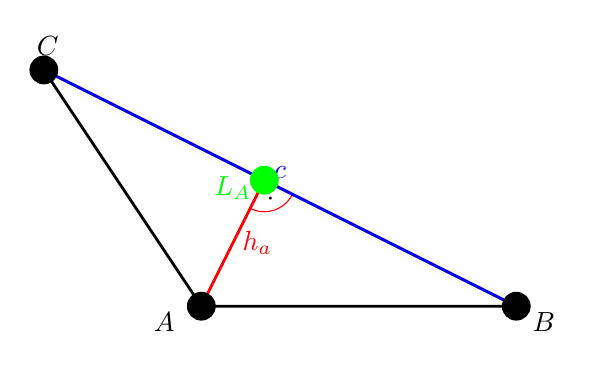
\begin{tikzpicture}
    \tkzSetUpPoint[shape=circle,size=10,color=black,fill=black]
    \tkzSetUpLine[line width=1]
    \tkzDefPoints{0/0/A, 4/0/B, -2/3/C}

    \tkzDefLine[orthogonal=through A,/tikz/overlay](B,C) \tkzGetPoint{helper}
    \tkzInterLL(B,C)(A,helper) \tkzGetPoint{La}

    \tkzMarkAngle[arc=l,size=0.4cm,color=red,fill=red!20](A,La,B)
    \tkzLabelAngle[pos=0.25](A,La,B){$\cdot$}

    \tkzDrawPolygon(A,B,C)

    \node at ($(A)+(-0.47,-0.2)$){$A$};
    \node at ($(B)+(0.35,-0.2)$) {$B$}; % \tkzLabelPoint[below](B){$B$} is not accurate enough
    \node at ($(C)+(0.05,0.3)$)  {$C$};
    \node[green] at ($(La)+(-0.4,-0.1)$)  {$L_A$};

    \tkzDrawSegments[red](A,La)
    \tkzDrawSegments[blue](B,C)
    \tkzLabelSegment[right,red](A,La){$h_a$}
    \tkzLabelSegment[above,blue](B,C){$c$}
    \tkzDrawPoints(A,B,C)
    \tkzDrawPoints[color=green,fill=green](La)
\end{tikzpicture}
\end{document}
